%
% einleitung.tex -- Beispiel-File für die Einleitung
%
% (c) 2020 Prof Dr Andreas Müller, Hochschule Rapperswil
%
% !TEX root = ../../buch.tex
% !TEX encoding = UTF-8
%
\section{Ein Moderner Beweis}
\label{basel:section:moderner-beweis}

Betrachtet wird die Funktion $x \mapsto x^2$ auf $[-\pi, \pi)$.
Zur Analyse dieser Funktion eignet sich die Fourier-Analyse besonders gut.
Die Darstellung von Funktionen als unendliche Summen von trigonometrischen
Funktionen ist etwas, worüber Euler auch schon nachgedacht hat, aber er kam nie
so weit, dass man hier von einer Theorie sprechen konnte.

\begin{figure}
\centering
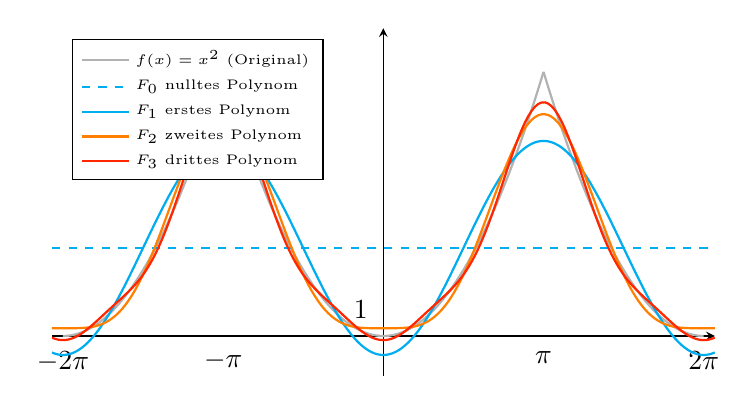
\begin{tikzpicture}
\begin{axis}[
    width=10cm, height=6cm,
    xmin=-6.5, xmax=6.5,
    ymin=-1.5, ymax=11.5,
    xtick={-6.2832,-3.1416,0,3.1416,6.2832},
    xticklabels={$-2\pi$,$-\pi$,$0$,$\pi$,$2\pi$},
    ytick={1},
    axis lines=center,
    tick style={draw=none},
    legend pos=north west,
    legend style={font=\tiny, cells={anchor=west}},
    %axis background/.style={fill=white},
    %legend style={fill=white, draw=black}, (ANSICHTSPROBLEM MIT DER SEITENFARBE?!?!)
]
\addplot[gray!60, thick, domain=-3.1416:3.1416, samples=100, forget plot] {x^2};
\addplot[gray!60, thick, domain=-6.2832:-3.1416, samples=100, forget plot] {(x+6.2832)^2};
\addplot[gray!60, thick, domain=3.1416:6.2832, samples=100] {(x-6.2832)^2};
\addlegendentry{$f(x)=x^2$ (Original)}
\addplot[cyan, dashed, thick, domain=-6.5:6.5] {3.2899};
\addlegendentry{$F_0$ nulltes Polynom}
\addplot[cyan, thick, domain=-6.5:6.5, samples=200]
    {3.2899 + 4*(-1)*cos(deg(x))};
\addlegendentry{$F_1$ erstes Polynom}
\addplot[orange, thick, domain=-6.5:6.5, samples=200]
    {3.2899 + 4*(-1)*cos(deg(x)) + 4*(0.25)*cos(deg(2*x))};
\addlegendentry{$F_2$ zweites Polynom}
\addplot[red!70!orange, thick, domain=-6.5:6.5, samples=200]
    {3.2899 + 4*(-1)*cos(deg(x)) + 4*(0.25)*cos(deg(2*x))
     + 4*(-0.1111)*cos(deg(3*x))};
\addlegendentry{$F_3$ drittes Polynom}
\end{axis}
\end{tikzpicture}
\caption{Periodische Fortsetzung von $f(x) = x^2$ mit den Fourierpolynomen
$F_0$ bis $F_3$.}
\end{figure}

Das nullte Fourierpolynom dieser Funktion ist nicht besonders, denn es handelt sich
lediglich um eine konstante Funktion.
Anhand der Beobachtung dieser Polynome wird deutlich, dass die Näherung immer
besser wird, wenn man die verschiedenen Polynomfunktionen betrachtet. Da die
Ausgangsfunktion jedoch nicht durchgehend differenzierbar ist, sind unendlich
viele Fourierpolynome erforderlich.
In dieser Hinsicht ist als Grundlage des Beweises das Theorem heranzuziehen,
das besagt, dass es zu punktweiser Konvergenz kommen wird, weil die Funktion
stetig ist.

\subsection{Berechnung der Fourierpolynome}
\label{basel:subsection:berechnung-fourierpolynome}

\begin{figure}
\centering
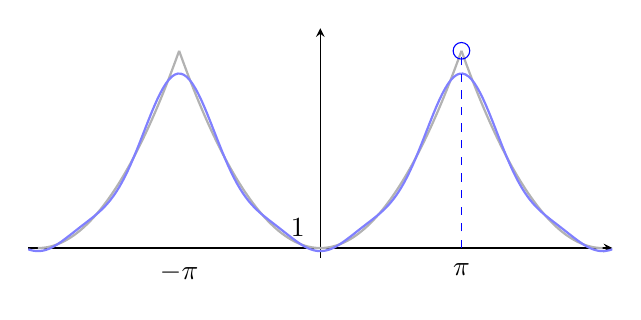
\begin{tikzpicture}
\begin{axis}[
    width=9cm, height=4.5cm,
    xmin=-6.5, xmax=6.5,
    ymin=-0.5, ymax=11,
    xtick={-3.1416, 3.1416},
    xticklabels={$-\pi$, $\pi$},
    ytick={1},
    axis lines=center,
    tick style={draw=none},
]
\addplot[gray!60, thick, domain=-3.1416:3.1416, samples=100] {x^2};
\addplot[gray!60, thick, domain=-6.2832:-3.1416, samples=100] {(x+6.2832)^2};
\addplot[gray!60, thick, domain=3.1416:6.2832, samples=100] {(x-6.2832)^2};
\addplot[blue!50, thick, domain=-6.5:6.5, samples=200]
    {3.2899 + 4*(-1)*cos(deg(x)) + 4*(0.25)*cos(deg(2*x))
     + 4*(-0.1111)*cos(deg(3*x))};
\addplot[blue, only marks, mark=o, mark size=3pt]
    coordinates {(3.1416, 9.8696)};
\draw[blue, dashed] (axis cs:3.1416,0) -- (axis cs:3.1416,9.8696);
\end{axis}
\end{tikzpicture}
\caption{Im Punkt $\pi$ liegt Konvergenz gegen den Funktionswert $\pi^2$ vor.}
\end{figure}

Ausgangspunkt der Analyse ist die Funktion
\[
f(x) = x^2.
\]
Das allgemeine Fourierpolynom der Ordnung $n$ ist
\[
F_n f(x)
=
\frac{a_0}{2}
+
\sum_{k=1}^{n}
\bigl(
a_k \cos(kx) + b_k \sin(kx)
\bigr).
\]
Da $f(x) = x^2$ eine gerade Funktion ist, verschwinden alle Sinus-Koeffizienten:
\[
b_k
=
\frac{1}{\pi}
\int_{-\pi}^{\pi} x^2 \sin(kx)\, dx
=
0,
\quad (k > 0).
\]
Der Koeffizient $a_0$ ergibt sich zu
\[
a_0
=
\frac{1}{\pi}
\int_{-\pi}^{\pi} x^2\, dx
=
\left.
\frac{x^3}{3\pi}
\right|_{-\pi}^{\pi}
=
\frac{2\pi^2}{3}.
\]
Für $k > 0$ liefert partielle Integration
\begin{align*}
a_k
&=
\frac{1}{\pi}
\int_{-\pi}^{\pi} x^2 \cos(kx)\, dx
\\
&=
\frac{1}{k\pi}
\left(
\left.
x^2 \sin(kx)
\right|_{-\pi}^{\pi}
-
2 \int_{-\pi}^{\pi} x \sin(kx)\, dx
\right)
\\
&=
-\frac{2}{k\pi}
\int_{-\pi}^{\pi} x \sin(kx)\, dx
\\
&=
\frac{2}{k^2\pi}
\left(
\left.
x \cos(kx)
\right|_{-\pi}^{\pi}
-
\int_{-\pi}^{\pi} \cos(kx)\, dx
\right)
\\
&=
\left.
\frac{2x}{k^2\pi} \cos(kx)
\right|_{-\pi}^{\pi}
=
(-1)^k \frac{4}{k^2},
\quad (k > 0).
\end{align*}
Damit ergibt sich die Fourierreihe von $f$:
\[
f(x)
=
\frac{a_0}{2}
+
\sum_{k=1}^{\infty}
\bigl(
a_k \cos(kx) + b_k \sin(kx)
\bigr)
=
\frac{\pi^2}{3}
+
4 \sum_{k=1}^{\infty} \frac{(-1)^k}{k^2} \cos(kx).
\]
Setzt man nun $\pi^2 = f(\pi)$ ein, so erhält man
\begin{equation}
\pi^2
=
f(\pi)
=
\frac{\pi^2}{3}
+
4 \sum_{k=1}^{\infty} \frac{(-1)^k}{k^2} \cos(k\pi)
=
\frac{\pi^2}{3}
+
\sum_{k=1}^{\infty} \frac{4}{k^2}.
\label{basel:equation:fourier-einsetzen}
\end{equation}
